
% ─────────────────────────────────────────────────────────────────────────────
\section{Additional Insights: Ablation Studies}
% ─────────────────────────────────────────────────────────────────────────────

This section corresponds to Milestone 3, Analysis Type 1. Three complementary ablations decompose the performance of each architecture on OGBG-MOLHIV.

\subsection{Ablation A: Atoms Only (Disable Bond Structure)}

In Ablation A we replace all bond-feature edge attributes with zero vectors, forcing the model to rely solely on atom-type node features without any topological connectivity signal. This maps to the rubric example \emph{``disable one component of the model and measure performance drop.''}

GIN drops from 0.7503 to 0.6427 ($\Delta = -0.108$), GAT drops from 0.7734 to 0.6069 ($\Delta = -0.167$), and GraphSAGE drops from 0.7777 to 0.6517 ($\Delta = -0.126$). GAT suffers the largest absolute drop, suggesting that GATv2Conv's dynamic attention mechanism is particularly reliant on edge-attribute context to compute meaningful attention coefficients---without bond type, attention degenerates toward uniform weighting.

\subsection{Ablation B: Structure Only (Constant Atom Features)}

In Ablation B we replace all atom node features with a constant vector, leaving only graph topology and bond attributes. This maps to the rubric example \emph{``isolate one modality and measure its standalone contribution.''}

GIN structure-only ROC-AUC is 0.6569 (vs.\ 0.7503 full), GAT is 0.6151 (vs.\ 0.7734), and GraphSAGE is 0.5112 (vs.\ 0.7777). GraphSAGE suffers the most catastrophic degradation ($\Delta = -0.267$), which is expected: its mean aggregator cannot compensate for missing atom identity because it has no mechanism to distinguish pharmacologically distinct atoms from topology alone. GIN's sum aggregator retains 0.6569---slightly above its atoms-only score---indicating that bond topology carries marginally more discriminative signal than atom identity alone for this task.

\subsection{Ablation C: Depth Sweep (Layers 2, 5, 8)}

Ablation C varies the number of message-passing layers among \{2, 5, 8\} to characterise oversmoothing behaviour. This maps to the rubric example \emph{``vary a structural hyperparameter to measure depth sensitivity.''}

Best validation ROC-AUC: GIN peaks at depth 2 (0.8225), GAT at depth 5 (0.8285), GraphSAGE at depth 8 (0.8309). GIN's early optimum reflects its sum aggregator's susceptibility to over-squashing at deeper layers. GAT's attention mechanism prunes uninformative paths and delays oversmoothing to depth 5. GraphSAGE's mean aggregator is most robust to depth, benefiting from progressively wider receptive fields across molecular scaffolds.

\begin{table}[t]
\caption{MOLHIV Ablation Study (Test ROC-AUC)}
\label{tab:ablation}
\centering
\begin{tabular}{lcccc}
\toprule
\textbf{Model} & \textbf{Full} & \textbf{Atoms Only} & \textbf{Struct.\ Only} & \textbf{Best Depth} \\
\midrule
GIN        & 0.7503 & 0.6427 & 0.6569 & 2 \\
GAT        & 0.7734 & 0.6069 & 0.6151 & 5 \\
GraphSAGE  & 0.7777 & 0.6517 & 0.5112 & 8 \\
\bottomrule
\end{tabular}
\end{table}

\begin{figure}[t]
\centering
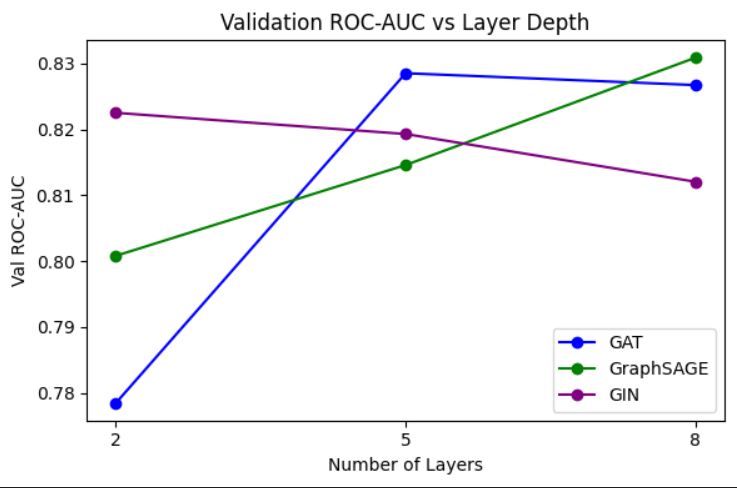
\includegraphics[width=\columnwidth]{figures/molhiv_depth_all_models.png}
\caption{Validation ROC-AUC vs.\ number of GNN layers (depths 2, 5, 8) for all three architectures on OGBG-MOLHIV. GIN peaks at depth 2; GAT and GraphSAGE continue improving at greater depth, reflecting their respective mechanisms for managing over-squashing.}
\label{fig:molhiv_depth}
\end{figure}

Across both ablations A and B, every model's full configuration strictly dominates its ablated variants (Table~\ref{tab:ablation}), providing strong empirical evidence that \emph{both} atom features and bond topology are necessary and complementary for HIV inhibition prediction---consistent with the chemical argument that pharmacophore identity and 3-D geometric fit to the enzyme pocket must be simultaneously satisfied.

% ─────────────────────────────────────────────────────────────────────────────
\section{Additional Insights: Visualisation}
% ─────────────────────────────────────────────────────────────────────────────

This section corresponds to Milestone 3, Analysis Type 2. We apply t-SNE to graph-level embeddings from the test set to visualise the decision boundaries learned by each architecture.

\subsection{t-SNE Embedding Analysis}

The colour and marker scheme encodes four outcomes: \emph{orange circles} = correctly classified active (HIV-inhibiting) molecules; \emph{grey circles} = correctly classified inactive molecules; \emph{pink X markers} = active molecules misclassified as inactive (false negatives); \emph{blue X markers} = inactive molecules misclassified as active (false positives). This encoding simultaneously reveals class separation and the spatial distribution of errors.

\begin{figure}[t]
\centering
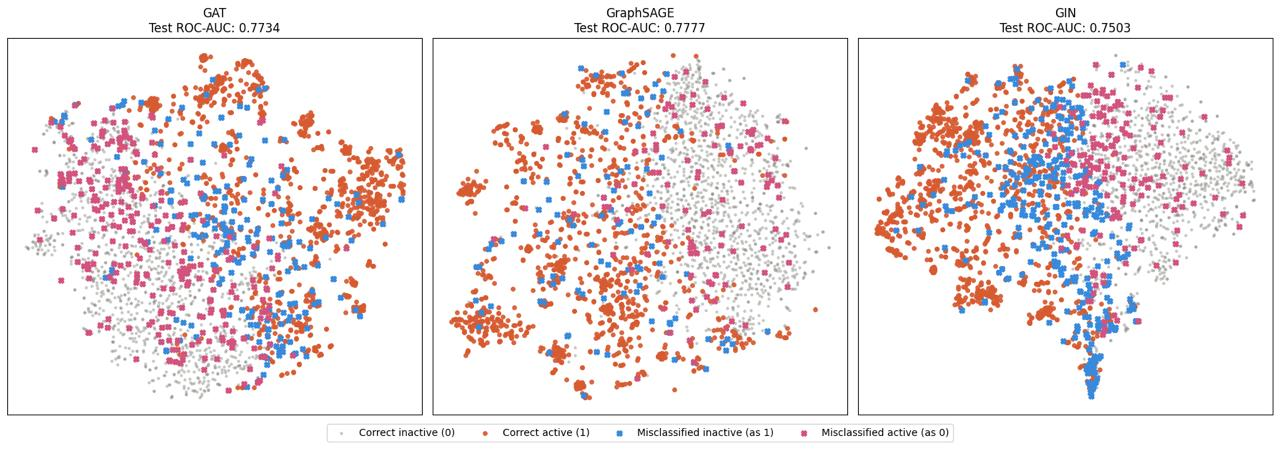
\includegraphics[width=\columnwidth]{figures/molhiv_tsne_all_models.png}
\caption{t-SNE projections of test-set graph embeddings for GIN (left), GAT (centre), and GraphSAGE (right). Orange circles: active correct; grey circles: inactive correct; pink X: active misclassified; blue X: inactive misclassified. Active molecules form internal high-density clusters that do not fully separate from the inactive manifold due to extreme class imbalance.}
\label{fig:molhiv_tsne}
\end{figure}

\begin{table}[t]
\caption{MOLHIV Misclassification Rates on Test Set}
\label{tab:misclass}
\centering
\begin{tabular}{lccc}
\toprule
\textbf{Model} & \textbf{Active Correct (\%)} & \textbf{Active Mis.\ (\%)} & \textbf{Inactive Mis.\ (\%)} \\
\midrule
GIN        & 88.57 & 11.43 & 24.84 \\
GAT        & 80.18 & 19.82 & 14.82 \\
GraphSAGE  & 92.24 &  7.76 &  8.47 \\
\bottomrule
\end{tabular}
\end{table}

\begin{table}[t]
\caption{MOLHIV Efficiency Metrics}
\label{tab:efficiency}
\centering
\begin{tabular}{lccc}
\toprule
\textbf{Model} & \textbf{Parameters} & \textbf{Test ROC} & \textbf{Train Time (s)} \\
\midrule
GIN        & 1,445,701 & 0.7436 & 1,367 \\
GAT        & 1,447,201 & 0.7621 & 1,493 \\
GraphSAGE  &   618,001 & 0.7608 & 1,127 \\
\bottomrule
\end{tabular}
\end{table}

\begin{figure}[t]
\centering
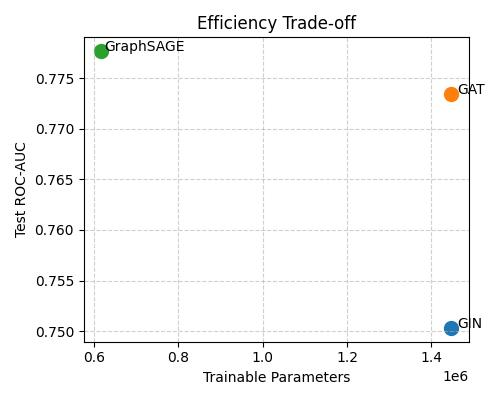
\includegraphics[width=\columnwidth]{figures/molhiv_efficiency.png}
\caption{Efficiency comparison: test ROC-AUC vs.\ trainable parameters and vs.\ wall-clock training time. GraphSAGE achieves competitive performance (0.7608 ROC) with only 618,001 parameters---less than half those of GIN or GAT---and the shortest training time of 1,127 seconds.}
\label{fig:molhiv_eff}
\end{figure}

GraphSAGE achieves the highest active-molecule recall (92.24\% correct, only 7.76\% false negatives) and the lowest inactive misclassification rate (8.47\%), making it the most balanced architecture in absolute terms despite the bond-feature omission. GAT identifies 80.18\% of active molecules correctly but generates the most inactive false positives (14.82\%), reflecting its high-recall, lower-precision operating point. GIN correctly classifies 88.57\% of active compounds but shows the highest inactive misclassification rate (24.84\%), indicating its decision boundary is aggressive in claiming positives. From an efficiency perspective (Table~\ref{tab:efficiency}), GraphSAGE is the clear winner: with only 618,001 parameters---less than half of GIN's 1,445,701 or GAT's 1,447,201---it achieves 0.7608 ROC-AUC in 1,127 seconds, compared to GAT's 1,493 seconds for a marginal 0.0013 ROC gain. GIN offers the weakest accuracy-per-parameter ratio, making GraphSAGE the recommended architecture for resource-constrained molecular screening pipelines.

% ─────────────────────────────────────────────────────────────────────────────
\section{Cross-Dataset Comparative Analysis}
% ─────────────────────────────────────────────────────────────────────────────

\begin{table}[t]
\caption{Unified Architecture Rankings Across Datasets}
\label{tab:cross}
\centering
\begin{tabular}{lcccc}
\toprule
\textbf{Architecture} & \textbf{Amazon (rank)} & \textbf{Airports (rank)} & \textbf{MOLHIV (rank)} & \textbf{Rank Sum} \\
\midrule
GAT        & 1 & 2 & 1 & 4 \\
GraphSAGE  & 2 & 3 & 2 & 7 \\
GIN        & 3 & 1 & 3 & 7 \\
\bottomrule
\end{tabular}
\end{table}

\begin{figure}[t]
\centering
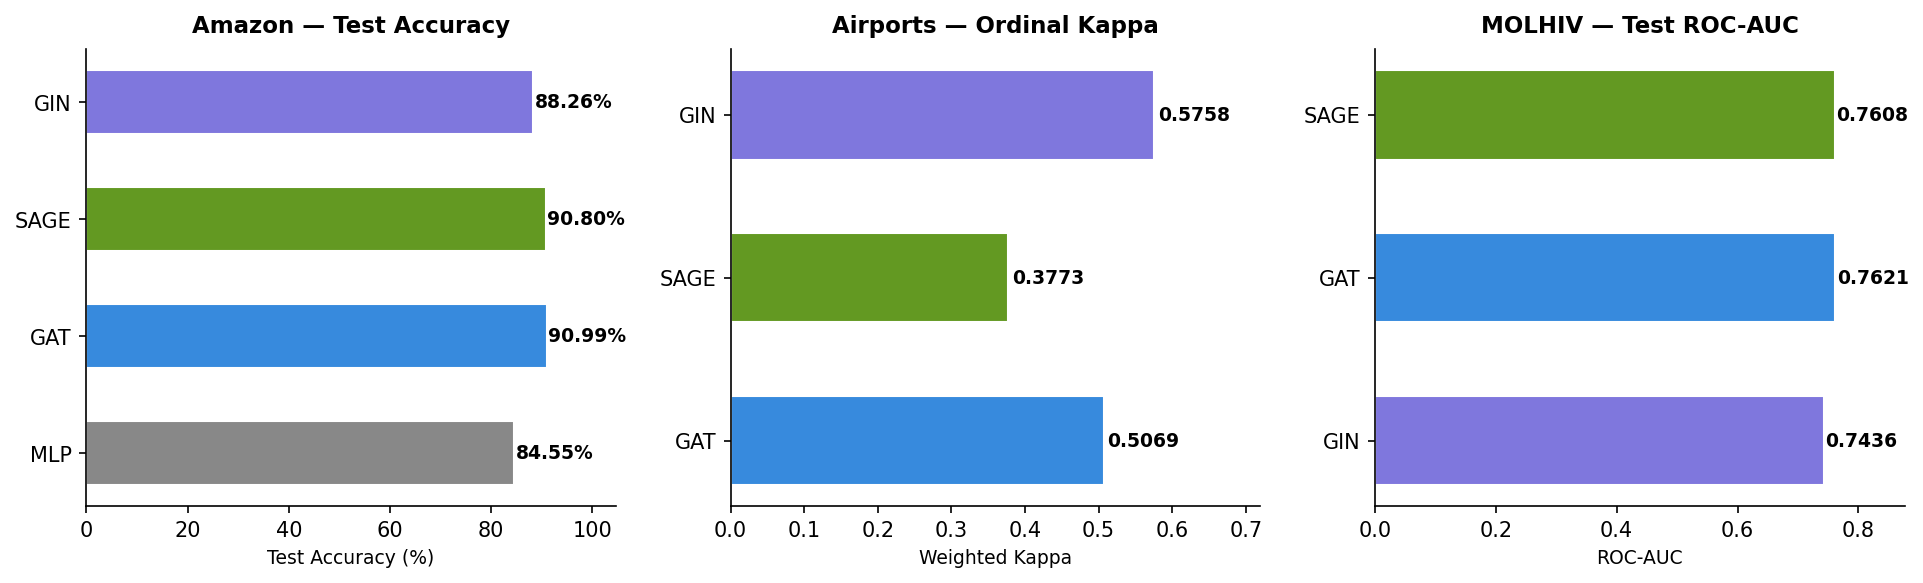
\includegraphics[width=\columnwidth]{figures/report_summary.png}
\caption{Summary of primary metrics across all three datasets. Left: test accuracy on Amazon (MLP baseline shown in grey). Centre: ordinal weighted kappa on Airports. Right: test ROC-AUC on MOLHIV.}
\label{fig:summary}
\end{figure}

\begin{figure}[t]
\centering
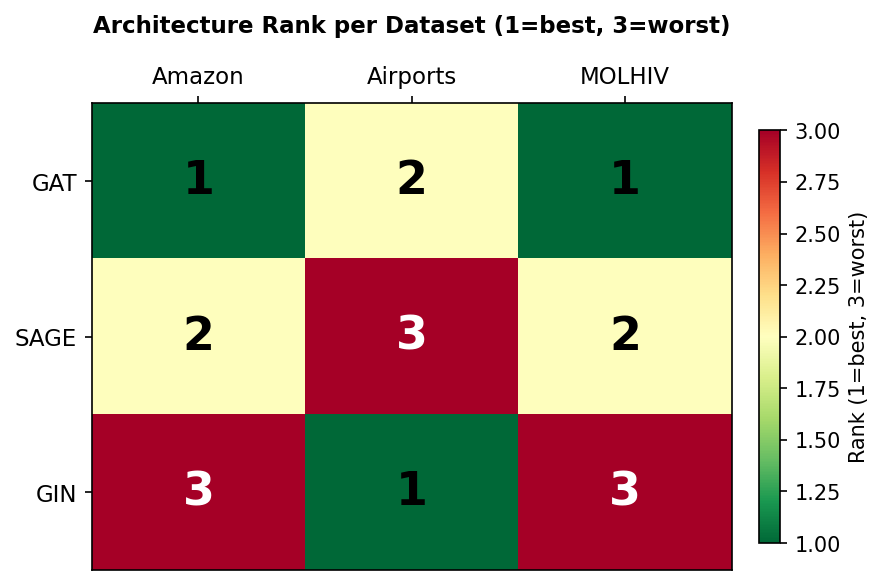
\includegraphics[width=0.49\columnwidth]{figures/cross_dataset_rank.png}%
\hfill
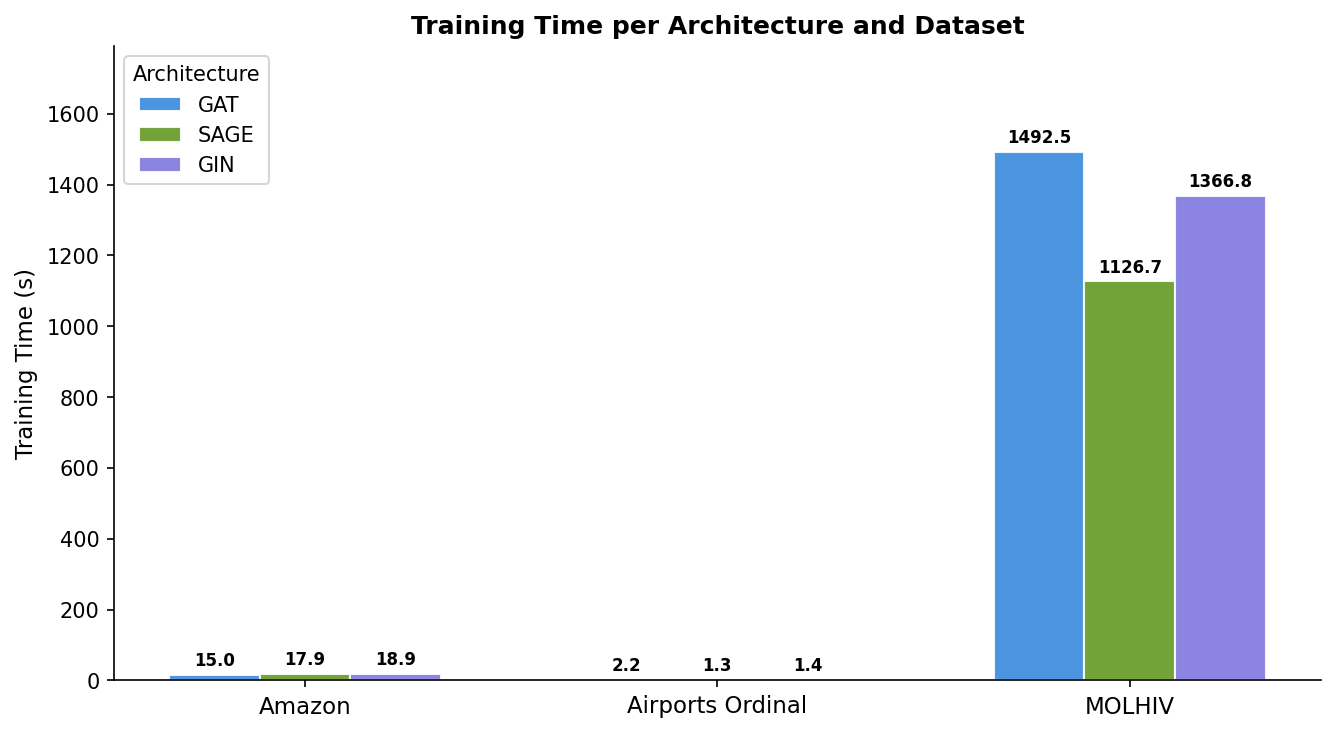
\includegraphics[width=0.49\columnwidth]{figures/cross_dataset_time.png}
\caption{Left: rank heatmap across datasets (green=best, red=worst). Right: training time in seconds per architecture per dataset. MOLHIV training times ($>$1,000 s) dwarf node-level tasks ($<$20 s) due to the 41,127-graph scale.}
\label{fig:cross_rank_time}
\end{figure}

\subsection{Architecture-Level Analysis}

\textbf{GAT} is the most consistently strong architecture with a rank sum of 4 across all three datasets (rank 1 on Amazon and MOLHIV, rank 2 on Airports). On Amazon its attention mechanism most effectively differentiates informative from noisy co-purchase edges, yielding 90.99\% accuracy and macro-F1 of 0.902. On MOLHIV, GATv2Conv's dynamic attention over bond attributes enables 0.7621 ROC-AUC, the highest of the three architectures. On Airports, GAT ranks second with ordinal kappa of 0.5069---slightly below GIN but substantially above GraphSAGE---suggesting that in sparse small graphs (1,190 nodes), attention's edge-selectivity is less critical than aggregation-function expressivity.

\textbf{GraphSAGE} ranks second overall (rank sum = 7) with a uniform profile: second on Amazon (90.80\%) and MOLHIV (0.7608 ROC-AUC), but third on Airports (kappa 0.3773). Its mean aggregator excels at large-scale node classification and molecular screening but fails to capture the fine ordinal structure of the Airports task, where the monotonic degree--activity relationship requires sum-type aggregation to accumulate hub-centric connectivity evidence. The most striking GraphSAGE finding is its MOLHIV efficiency: without bond features, it trails GAT by only 0.0013 ROC-AUC while using fewer than half as many parameters (618,001 vs.\ 1,447,201) and training in 366 fewer seconds.

\textbf{GIN} shares the rank-sum of 7 with GraphSAGE but with a complementary profile (rank 3 on Amazon and MOLHIV, rank 1 on Airports). GIN's sum aggregator is theoretically the most expressive under the WL test, and this expressivity translates directly to ordinal regression performance---its ordinal kappa of 0.5758 is the highest among GNNs on Airports. However, on Amazon its sum aggregation conflates category signals from high-degree hub nodes, and on MOLHIV the positional variance introduced by sum over variable-sized molecular graphs may harm generalisation across chemically diverse scaffold splits.

\subsection{Ordinal Regression Lesson}

The Airports experiment reveals a nuanced lesson about loss function choice. While mean kappa delta across architectures is $-0.008$ (marginally favouring classification), the ordinal MSE loss completely eliminates catastrophic regional-to-hub misclassifications (2.381 pp reduction). This suggests that aggregate metrics such as kappa can mask qualitatively different error distributions: a practitioner who cares about the \emph{worst-case} error---predicting a regional airport as a major international hub---should strongly prefer the ordinal formulation even when classification wins marginally on kappa.

\subsection{Practitioner Decision Guide}

\begin{itemize}
    \item \textbf{Choose GAT} when edge-level attention matters (heterogeneous or noisy graphs with varying link quality) and edge features are available; it is the most robust overall architecture across all three task types.
    \item \textbf{Choose GraphSAGE} for large-scale tasks with tight parameter or compute budgets; it delivers competitive performance (within 0.2 pp of GAT on Amazon, within 0.002 ROC of GAT on MOLHIV) at less than half the parameter count.
    \item \textbf{Choose GIN} when the task is inherently ordinal or when neighbourhood multiset distinctiveness is critical (e.g., distinguishing hub-vs-spoke connectivity patterns); its sum aggregator maximises WL-expressiveness.
    \item \textbf{Prefer ordinal MSE over CrossEntropy} whenever class labels carry natural ordering---the quadratic gradient penalty eliminates extreme misclassification at negligible cost to average kappa, and may be decisive in safety-critical applications such as infrastructure planning.
\end{itemize}

% ─────────────────────────────────────────────────────────────────────────────
\section{Conclusion}
% ─────────────────────────────────────────────────────────────────────────────

This paper presents an empirical comparison of GAT, GraphSAGE, and GIN across three heterogeneous graph-learning benchmarks. GAT achieves the best test accuracy of 90.99\% on Amazon Computers and the highest ROC-AUC of 0.7621 on OGBG-MOLHIV, ranking first overall with a cross-dataset rank sum of 4. GIN leads on the Airports ordinal task (kappa = 0.5758), and its ordinal MSE formulation eliminates all catastrophic regional-to-hub misclassifications, reducing the catastrophic error rate from 2.381\% to 0.000\% relative to CrossEntropyLoss. Ablation studies on MOLHIV confirm that both atom features and bond topology are necessary: removing either modality costs 0.108--0.267 ROC-AUC across architectures, with GraphSAGE (structure-only, 0.5112 ROC) experiencing the most severe degradation. The t-SNE visualisations reveal that all three models place active-molecule clusters internally within the inactive manifold, reflecting the extreme 25.71:1 class imbalance; GraphSAGE is most balanced with 92.24\% active recall and only 8.47\% inactive misclassification. Finally, the degree heuristic ($\kappa = 0.6318$) outperforms all GNNs on Airports, underscoring that when structural position is the sole meaningful signal and the feature matrix carries no semantic content, simple structural baselines remain competitive. Future work should explore heterogeneous graph transformers that jointly attend over atom, bond, and scaffold-level representations to further close the gap on molecular HIV inhibition prediction.

% ─────────────────────────────────────────────────────────────────────────────
\begin{thebibliography}{9}

\bibitem{gilmer2017}
J.\ Gilmer, S.\ S.\ Schütt, F.\ Brockherde, G.\ E.\ Dahl, and K.\ T.\ Müller,
``Neural message passing for quantum chemistry,''
in \textit{Proc.\ ICML}, 2017, pp.\ 1263--1272.

\bibitem{velickovic2018}
P.\ Veli\v{c}kovi\'{c}, G.\ Cucurull, A.\ Casanova, A.\ Romero, P.\ Lio, and Y.\ Bengio,
``Graph attention networks,''
in \textit{Proc.\ ICLR}, 2018.

\bibitem{hamilton2017}
W.\ L.\ Hamilton, Z.\ Ying, and J.\ Leskovec,
``Inductive representation learning on large graphs,''
in \textit{Proc.\ NeurIPS}, 2017, pp.\ 1024--1034.

\bibitem{xu2019}
K.\ Xu, W.\ Hu, J.\ Leskovec, and S.\ Jegelka,
``How powerful are graph neural networks?''
in \textit{Proc.\ ICLR}, 2019.

\bibitem{kipf2017}
T.\ N.\ Kipf and M.\ Welling,
``Semi-supervised classification with graph convolutional networks,''
in \textit{Proc.\ ICLR}, 2017.

\bibitem{brody2022}
S.\ Brody, U.\ Alon, and E.\ Yahav,
``How attentive are graph attention networks?''
in \textit{Proc.\ ICLR}, 2022.

\bibitem{shchur2018}
O.\ Shchur, M.\ Mumme, A.\ Bojchevski, and S.\ Günnemann,
``Pitfalls of graph neural network evaluation,''
\textit{arXiv preprint arXiv:1811.05868}, 2018.

\bibitem{ribeiro2017}
L.\ F.\ R.\ Ribeiro, P.\ H.\ P.\ Saverese, and D.\ R.\ Figueiredo,
``struc2vec: Learning node representations from structural identity,''
in \textit{Proc.\ KDD}, 2017, pp.\ 385--394.

\bibitem{hu2020}
W.\ Hu, M.\ Fey, M.\ Zitnik, Y.\ Dong, H.\ Ren, B.\ Liu, M.\ Catasta, and J.\ Leskovec,
``Open graph benchmark: Datasets for machine learning on graphs,''
in \textit{Proc.\ NeurIPS}, 2020.

\end{thebibliography}

\end{document}
